\section{Bootloader optimizations}

\begin{frame}
\frametitle{Bootloader}
\begin{itemize}

\item Remove unnecessary functionality.\\
      Usually, bootloaders include many features needed only for
      development. Compile your bootloader with less features.
\item Optimize required functionality.\\
      Tune your bootloader for fastest performance. \\
      Switch to another bootloader (if available) \\
      Skip the bootloader and load the kernel right away.
\end{itemize}
\end{frame}

\subsection{U-Boot optimizations}

\begin{frame}
\frametitle{U-Boot - Remove unnecessary functionality}
Recompile U-Boot to remove features not needed in production
\begin{itemize}
\item Disable as many features as possible 
      in \code{include/configs/<soc>-<board>.h}
\item Examples: MMC, USB, Ethernet, dhcp, ping, command line edition,
      command completion...
\item A smaller and simpler U-Boot is faster to load and faster 
      to initialize.
\end{itemize}
\end{frame}

\begin{frame}
\frametitle{U-Boot - Remove the boot delay}
\begin{itemize}
\item Remove the boot delay:\\
      \code{setenv bootdelay 0}
\item This usually saves several seconds!
\item Before you do that, recompile U-Boot with
      \code{CONFIG_ZERO_BOOTDELAY_CHECK}, documented in
      \code{doc/README.autoboot}. It allows to stop the autoboot 
      process by hitting a key even if the boot delay is set to
      \code{0}.
\end{itemize}
\end{frame}

\begin{frame}
\frametitle{U-Boot - Optimize kernel loading}
\begin{itemize}
\item After copying the kernel \code{uImage} to RAM,
      U-Boot always moves it to the load address specified
      in the \code{uImage} header.
\item A CRC check is also performed.
\end{itemize}
\begin{center}
    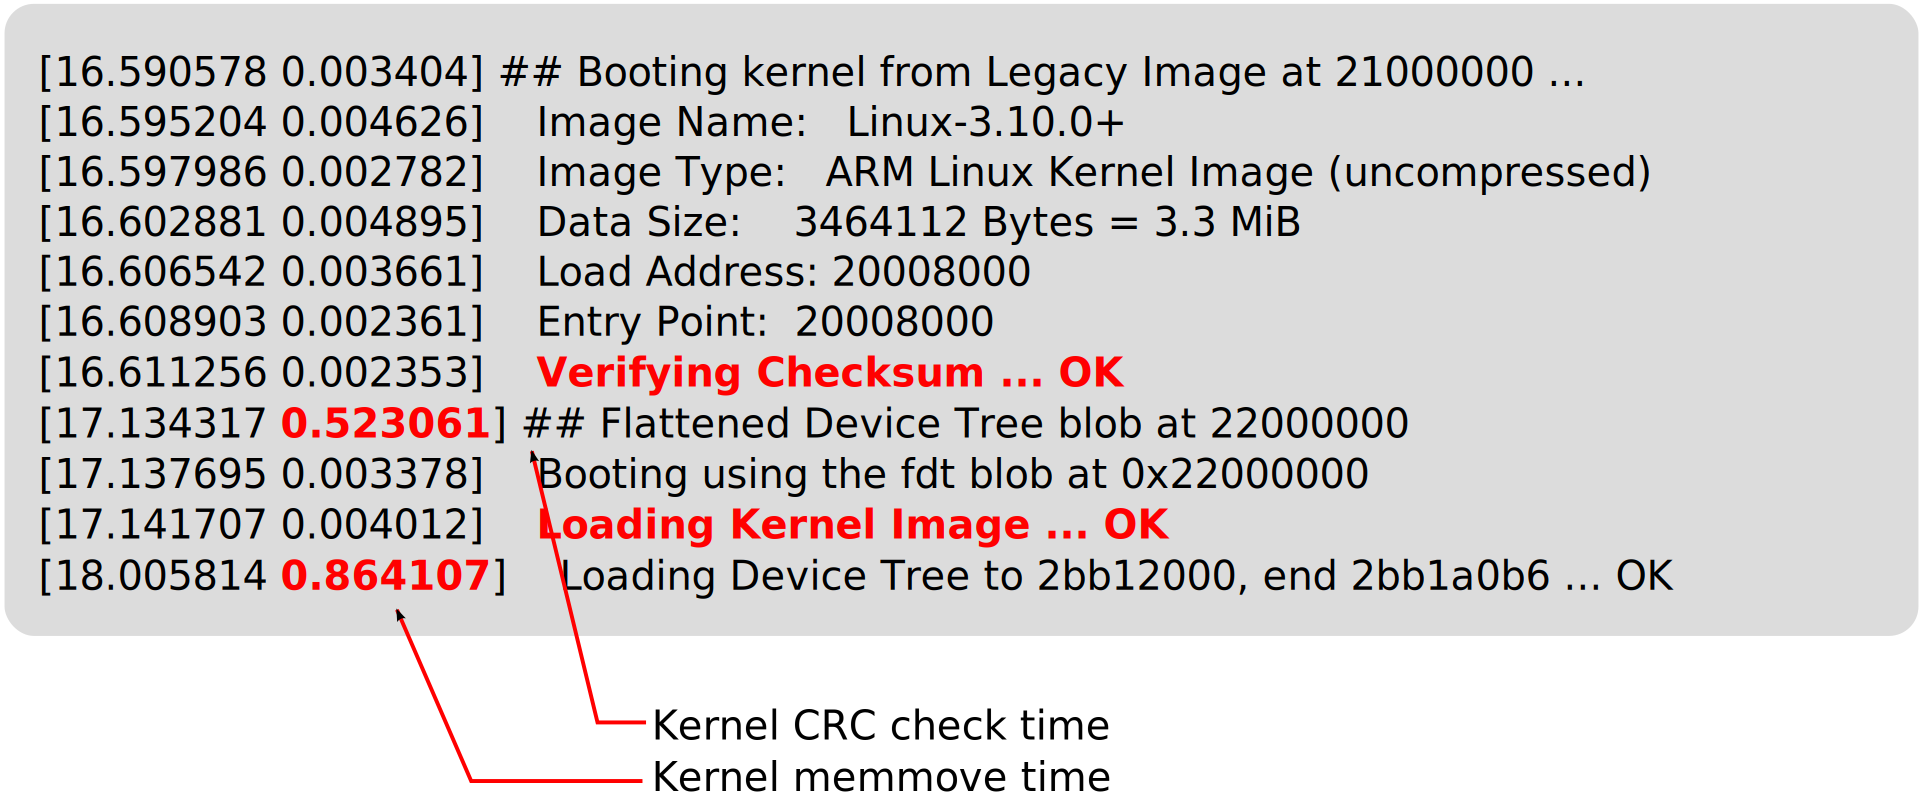
\includegraphics[width=\textwidth]{slides/boottime-bootloader/u-boot-kernel-loading.pdf}
\end{center}
\end{frame}

\begin{frame}
\frametitle{U-Boot - Remove unnecessary memmove (1)}
\begin{itemize}
\item You can make U-Boot skip the \code{memmove} operation
      by directly loading the \code{uImage} at the right
      address.
\item Compute this address: \\
      {\small
      \code{Addr = Load Address - uImage header size}\\
      \code{Addr = Load Address - (size(uImage) - size(zImage))}\\ 
      \code{Addr = 0x20008000 - 0x40 = 0x20007fc0}\\
      }
\end{itemize}
\begin{center}
    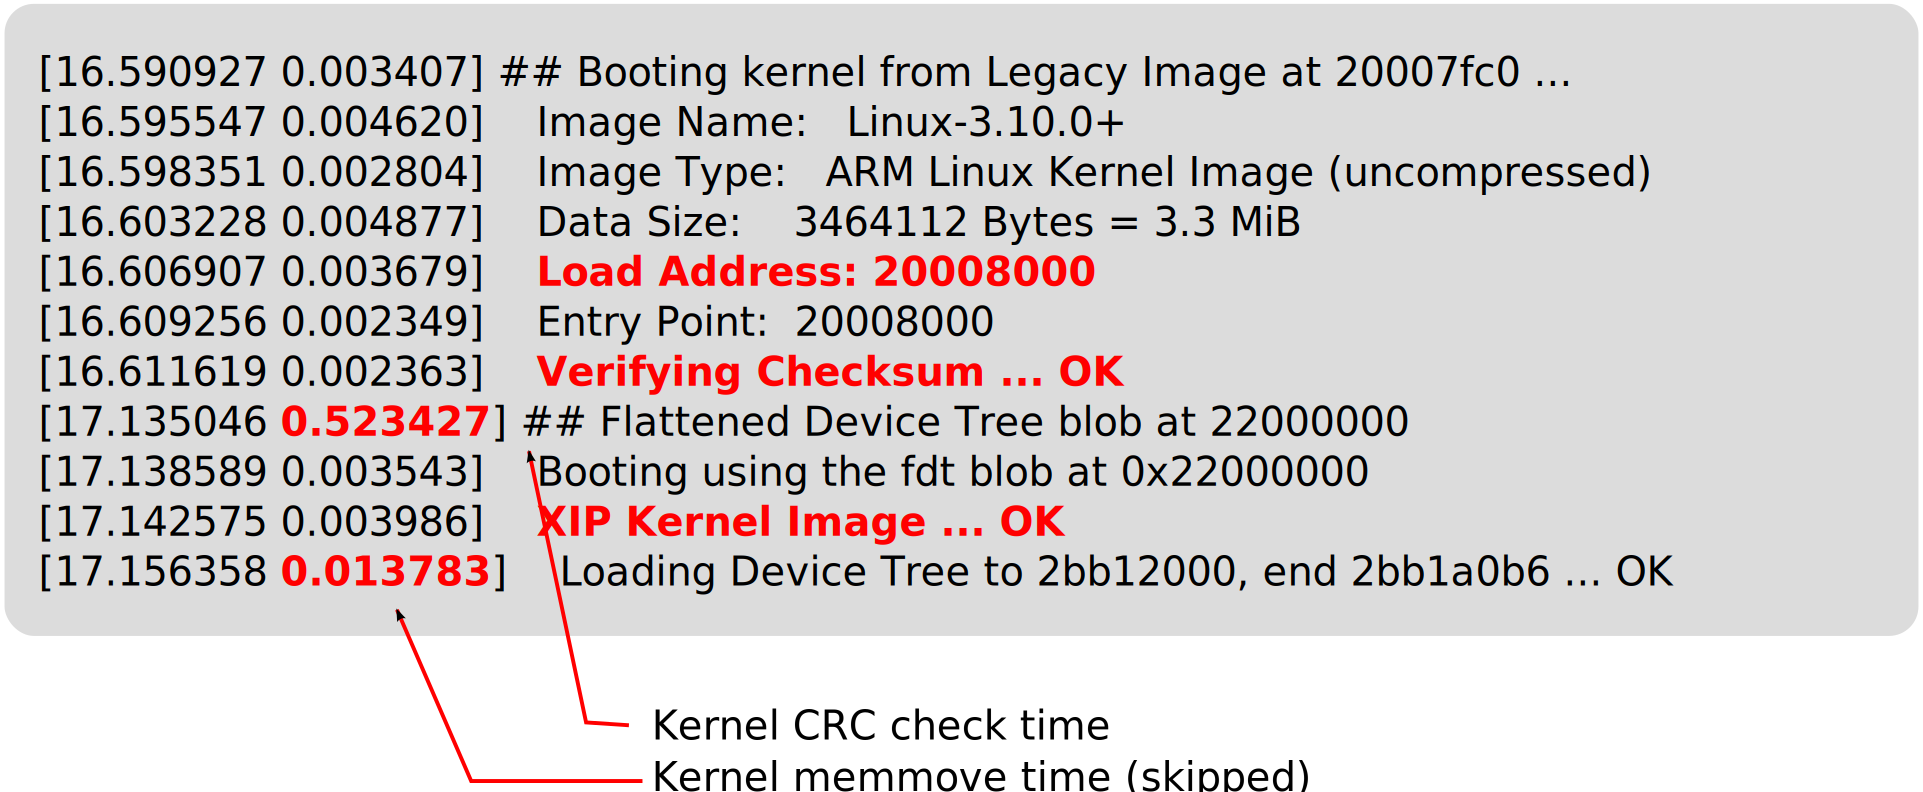
\includegraphics[width=\textwidth]{slides/boottime-bootloader/u-boot-kernel-loading-no-memmove.pdf}
\end{center}
\end{frame}

\begin{frame}
\frametitle{U-Boot - Remove unnecessary memmove (2)}
Results on Atmel SAMA5D3 Xplained (ARM), Linux 3.10:
\newline\newline
\begin{tabular}{| l || c | c |}
\hline
& Time & Diff \\
\hline
Default & 1.433 s & \\
Optimum load address & 0.583 s & -0.85 s\\
\hline
\end{tabular}
\newline\newline
\small
Measured between \code{Booting kernel} and \code{Starting kernel ...}
\end{frame}

\begin{frame}
\frametitle{U-Boot - Remove kernel CRC check}
\begin{itemize}
\item Fine in production when you no longer have data corruption
      copying the kernel to RAM.
\item Disable CRC checking with a U-boot environment variable:\\
      \code{setenv verify no}
\end{itemize}
Results on Atmel SAMA5D3 Xplained (ARM), Linux 3.10:
\newline\newline
\begin{tabular}{| l || c | c |}
\hline
& Time & Diff \\
\hline
With CRC check & 583 ms & \\
Without CRC check & 60 ms & -523 ms \\
\hline
\end{tabular}
\newline\newline
\small
Measured between \code{Booting kernel} and \code{Starting kernel ...}
\end{frame}

\begin{frame}
\frametitle{Further U-Boot optimizations}
\begin{itemize}
\item Silence U-Boot console output. You will need to compile
      U-Boot with \code{CONFIG_SILENT_CONSOLE} and
      \code{setenv silent yes}.\\
      See \code{doc/README.silent} for details.
\item Ultimate solution: use U-Boot's {\em Falcon} mode.\\
      U-Boot is split in two parts: the SPL (Secondary Program Loader)
      and the U-Boot image. U-Boot can then configure to the SPL to load
      the Linux kernel directly, instead of the U-Boot image.\\
      See \code{doc/README.falcon} for details.
\end{itemize}
\end{frame}

\subsection{Switching to another bootloader}

\begin{frame}
\frametitle{Switching from U-Boot to Barebox}
Results with the SAMA5D3x-EK board \\
Before: 5.77s
\begin{center}
    \includegraphics[width=\textwidth]{slides/boottime-kernel/timechart-final.pdf}
\end{center}
After:
\begin{center}
    \includegraphics[width=\textwidth]{slides/boottime-bootloader/timechart-barebox.pdf}
\end{center}
Total: 4.67s.
\end{frame}

\begin{frame}
\frametitle{Compression}
Let's try LZO compression for the kernel again:
Before (gzip): 4.67s
\begin{center}
    \includegraphics[width=\textwidth]{slides/boottime-bootloader/timechart-barebox.pdf}
\end{center}
After (LZO):
\begin{center}
    \includegraphics[width=\textwidth]{slides/boottime-bootloader/timechart-barebox-lzo.pdf}
\end{center}
Total: 4.59s.
\end{frame}

\begin{frame}[fragile]
\frametitle{Features}
Now, let's limit the features of the bootloader.\\
We still keep a way to interact with it when a GPIO has a given value.
For example, using the \code{gpio_direction_input} and
\code{gpio_get_value} commands in a script that would then start an
upgrade or boot a rescue kernel.
\begin{block}{}
\begin{verbatim}
gpio_get_value 42
if [ $? = 0 ]; then
    kdev="/dev/nand0.krescue.bb"
fi
\end{verbatim}
\end{block}
\end{frame}

\begin{frame}
\frametitle{Results}
Before: 4.59s
\begin{center}
    \includegraphics[width=\textwidth]{slides/boottime-bootloader/timechart-barebox-lzo.pdf}
\end{center}
After:
\begin{center}
    \includegraphics[width=\textwidth]{slides/boottime-bootloader/timechart-barebox-final.pdf}
\end{center}
Total: 3.07s.
\end{frame}

\begin{frame}
\frametitle{Results}
Note: the kernel didn't actually change but we don't get a message on
the serial line exactly at the time we switch from the bootloader to
the kernel.

Warning: Sometimes, the kernel is relying on the bootloader to
initialize the hardware (pinmuxing, clocks, ...) so be careful when
removing features.
\end{frame}

\begin{frame}
\frametitle{Results - Simplifying bootloader and kernel}

Before: 3.07s
\begin{center}
    \includegraphics[width=0.8\textwidth]{slides/boottime-bootloader/timechart-barebox-final.pdf}
\end{center}
After:
\begin{center}
    \includegraphics[width=0.8\textwidth]{slides/boottime-bootloader/timechart-kernel.pdf}
\end{center}
Total: 2.57s.
\end{frame}

\subsection{Skipping the bootloader}

\begin{frame}[fragile]
\frametitle{Removing the bootloader}
\begin{itemize}
\item Principle: instead of loading the bootloader and then the kernel,
      load the kernel right away!
\item For example, on Atmel AT91, is is easy to implement with
      \code{at91bootstrap v3}. You just need to configure it
      with one of the \code{linux} or \code{linux_dt} configurations:
\begin{block}{}
\begin{verbatim}
make at91sama5d3xeknf_linux_dt_defconfig
make
\end{verbatim}
\end{block}
      Full details on
      \url{http://free-electrons.com/blog/starting-linux-directly-from-at91bootstrap3/}

\item In our particular case, though, you will lose the
      main advantages of using Barebox.  It is uses the CPU caches
      while loading the kernel.
\end{itemize}
\end{frame}

\begin{frame}
\frametitle{Removing the bootloader}
Before: 3.07s
\begin{center}
    \includegraphics[width=\textwidth]{slides/boottime-bootloader/timechart-barebox-final.pdf}
\end{center}
Using \code{AT91bootstrap} to boot the Linux kernel:
\begin{center}
    \includegraphics[width=\textwidth]{slides/boottime-bootloader/timechart-at91.pdf}
\end{center}
Total: 3.94s.
\end{frame}

\setuplabframe
{Reduce bootloader time}
{
\begin{itemize}
\item Reduce boot time by using the Barebox bootloader
\item Optimize Barebox
\end{itemize}
}

